\chapter*{Proposition 36}



\begin{figure*}[ht]
    \begin{center}
    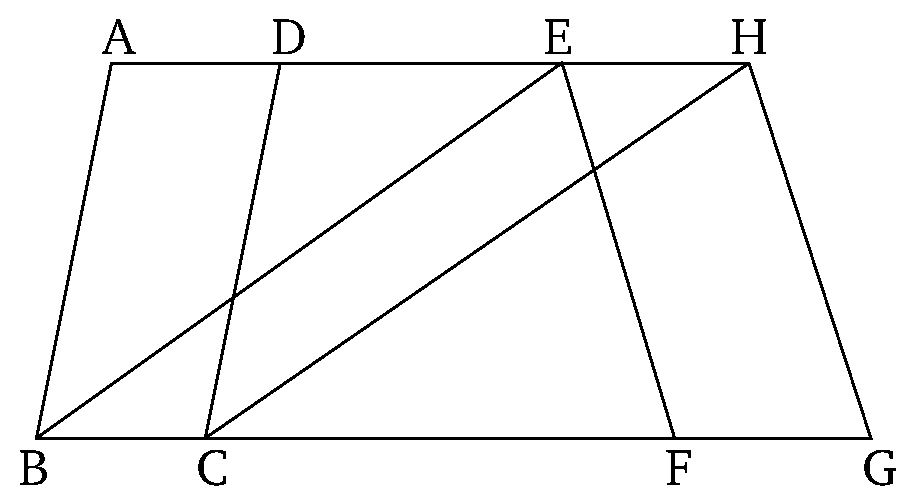
\includegraphics[width=0.5\linewidth]{figures/fig36e.eps}
    \label{fig:prop_36}
    \end{center}
\end{figure*}

Parallelograms which are on equal bases and between the same parallels are equal to one another.

Let $ABCD$ and $EFGH$ be parallelograms which are on the equal bases $BC$
and $FG$, and (are) between the same parallels $AH$ and $BG$. I say that
the parallelogram $ABCD$ is equal to $EFGH$.

For let $BE$ and $CH$ have been joined. And since $BC$ is equal to $FG$, but $FG$ is equal to $EH$ [Prop.~1.34], $BC$ is thus equal to $EH$. And they are also parallel, and $EB$ and $HC$ join them.
But (straight-lines) joining equal and parallel (straight-lines) on the
same sides are (themselves) equal and parallel [Prop.~1.33] [thus, $EB$ and $HC$
are also equal and parallel]. Thus, $EBCH$ is a parallelogram [Prop.~1.34],
and is equal to $ABCD$. For it has  the
same base, $BC$, as ($ABCD$), and is between the same parallels, $BC$ and $AH$, as ($ABCD$) [Prop.~1.35]. So,
for the same (reasons), $EFGH$ is also equal to the same (parallelogram) $EBCH$ [Prop.~1.34].  So that the
parallelogram $ABCD$ is  also equal to $EFGH$.

Thus, parallelograms which are on equal bases and between the same parallels are equal to one another. (Which is) the very thing it was required
to show.


\section*{Commentary}

\begin{proposition}\label{proposition_36}\lean{Elements.Book1.proposition_36}\leanok
    If
\end{proposition}
\begin{proof}
    \uses{proposition_33,proposition_34,proposition_35}\leanok
\end{proof}
